\chapter{Diseño e implementación}
\label{Chapter3}

\definecolor{mygreen}{rgb}{0,0.6,0}
\definecolor{mygray}{rgb}{0.5,0.5,0.5}
\definecolor{mymauve}{rgb}{0.58,0,0.82}

\lstset{ %
  backgroundcolor=\color{white},   % choose the background color; you must add \usepackage{color} or \usepackage{xcolor}
  basicstyle=\footnotesize,        % the size of the fonts that are used for the code
  breakatwhitespace=false,         % sets if automatic breaks should only happen at whitespace
  breaklines=true,                 % sets automatic line breaking
  captionpos=b,                    % sets the caption-position to bottom
  commentstyle=\color{mygreen},    % comment style
  deletekeywords={...},            % if you want to delete keywords from the given language
  %escapeinside={\%*}{*)},          % if you want to add LaTeX within your code
  %extendedchars=true,              % lets you use non-ASCII characters; for 8-bits encodings only, does not work with UTF-8
  %frame=single,	                % adds a frame around the code
  keepspaces=true,                 % keeps spaces in text, useful for keeping indentation of code (possibly needs columns=flexible)
  keywordstyle=\color{blue},       % keyword style
  language=[ANSI]C,                % the language of the code
  %otherkeywords={*,...},           % if you want to add more keywords to the set
  numbers=left,                    % where to put the line-numbers; possible values are (none, left, right)
  numbersep=5pt,                   % how far the line-numbers are from the code
  numberstyle=\tiny\color{mygray}, % the style that is used for the line-numbers
  rulecolor=\color{black},         % if not set, the frame-color may be changed on line-breaks within not-black text (e.g. comments (green here))
  showspaces=false,                % show spaces everywhere adding particular underscores; it overrides 'showstringspaces'
  showstringspaces=false,          % underline spaces within strings only
  showtabs=false,                  % show tabs within strings adding particular underscores
  stepnumber=1,                    % the step between two line-numbers. If it's 1, each line will be numbered
  stringstyle=\color{mymauve},     % string literal style
  tabsize=2,	                   % sets default tabsize to 2 spaces
  title=\lstname,                  % show the filename of files included with \lstinputlisting; also try caption instead of title
  morecomment=[s]{/*}{*/}
}

Este capítulo detalla la generación de contenido original del trabajo.
Se explica su diseño y producción.

\section{Autoevaluación del dispositivo bajo prueba}
\label{sec:autoevaluacion}

La construcción del \emph{firmware} de autoevaluación del dispositivo bajo prueba requirió superar las siguientes etapas:
\begin{itemize}
    \item Configuración de las señales de reloj del dispositivo bajo prueba.
    \item Selección y configuración de los periféricos del dispositivo bajo prueba.
    \item Selección y configuración de los terminales externos del dispositivo bajo prueba.
    \item Implementación de las estrategias de validación de periféricos.
    \item Integración de una secuencia de validación y reporte.
\end{itemize}

Para configurar las frecuencias de reloj se buscó obtener 150 MHz para suministrar al \emph{Master CAN Bus}.
Con esta condición satisfecha, se pudo configurar las frecuencias de reloj del resto de los periféricos.
En la figura \ref{fig:clock} se puede observar la utilización del \emph{Programmable Clock Controller} número cinco.

\begin{figure}[htbp]
	\centering
	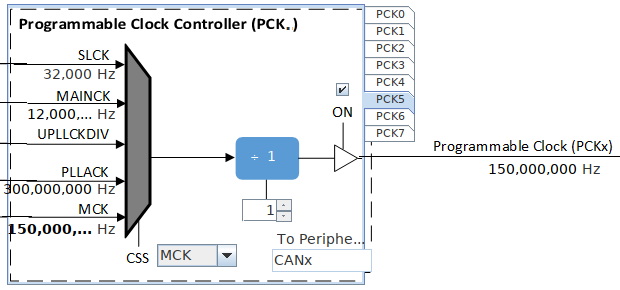
\includegraphics[width=\textwidth]{./Figures/Clock.png}
    \caption{Diagrama de configuración de las señales de reloj.}
	\label{fig:clock}
\end{figure}

El siguiente paso en la etapa de diseño fue la selección de las instancias de los periféricos del integrado.
Es posible que dos periféricos compartan parte del circuito interno o terminales del encapsulado.
Esta situación puede generar una disminución en las funcionalidades o una total incompatibilidad.
Finalmente, se seleccionaron instancias completamente disjuntas.

Luego de seleccionar las instancias de los periféricos, se configuraron para realizar un \emph{loopback}.
La configuración se realizó de la siguiente manera:

\begin{itemize}
    \item \emph{CAN}: se utilizó el \emph{MCAN1} con una configuración de \emph{loopback} interna, como se puede ver en la figura \ref{fig:canloopback}.
    \item \emph{PIO}: se configuraron dos terminales del dispositivo bajo prueba.
        El primero como salida sin \emph{latch} y el segundo como entrada sin circuito anti rebote.
    \item \emph{SPI}: la configuración elegida fue por defecto ya que el \emph{loopback} se logró conectando \emph{TX} y \emph{RX} con un cable.
    \item \emph{UART}: se configuró el periférico con una velocidad de 9600 baudios, 8 bits de datos y sin bits de paridad.
    \item \emph{Watchdog}: el disparo se configuró con un contador a 4095 cuentas.
        Este valor se estimó entre dos y cinco ejecuciones del \emph{loop} principal.
\end{itemize}

\begin{figure}[htbp]
	\centering
	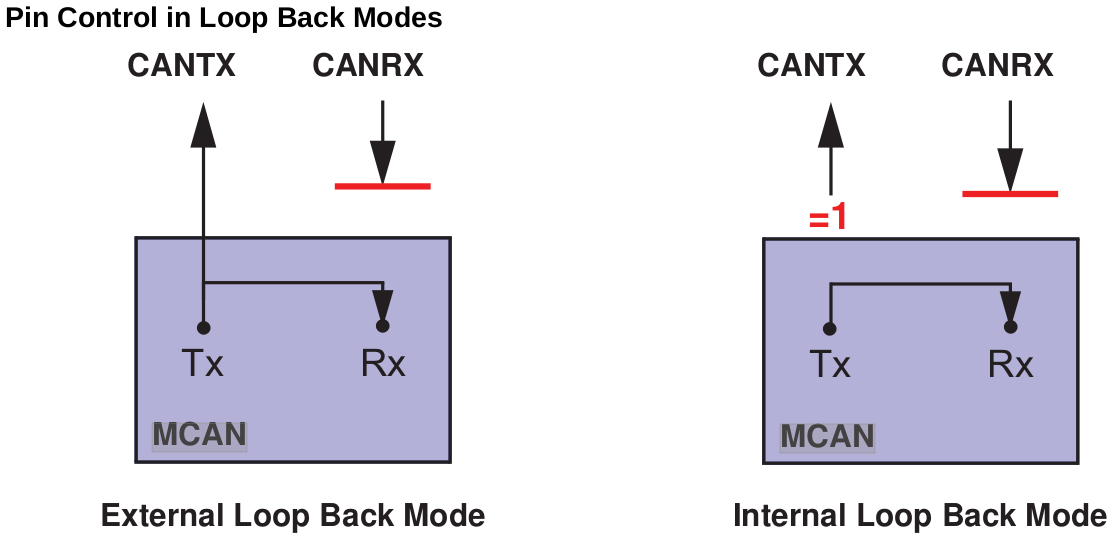
\includegraphics[width=0.8\textwidth]{./Figures/canloopback.png}
    \caption{Diagrama de \emph{loopback} del periférico \emph{CAN}\protect\footnotemark.}
	\label{fig:canloopback}
\end{figure}

\footnotetext{Imagen tomada de la hoja de datos del dispositivo bajo prueba \citep{ARTICLE:dutdatasheet}.}

Como se puede ver en la figura \ref{fig:labo}, se priorizaron los \emph{loopbacks} físicos externos.
Cuando esta estrategia no fue posible, se optó por internos provistos por el fabricante.
Finalmente, en los casos que las dos primeras opciones fuesen imposibles, se utilizó una estrategia de \emph{software}.
En la tabla \ref{tab:perifericos} se puede ver un resumen de las estrategias aplicadas.

\begin{table}[h]
	\centering
	\caption[Estrategias de depuración]{Comparación entre estrategias de depuración}

	\begin{tabular}{l c c}    
		\toprule
        \textbf{Periférico} & \textbf{Validación}       & \textbf{Detección en un ciclo}\\
		\midrule
		CAN                 & Loopback interno          & Si\\		
		PIO                 & Loopback externo          & No\\
		SPI                 & Loopback externo          & Si\\
		UART                & Lógica en firmware        & No\\
		Watchdog            & Lógica en inyector        & No\\
		\bottomrule
		\hline
	\end{tabular}
	\label{tab:perifericos}
\end{table}

\begin{figure}[htbp]
	\centering
	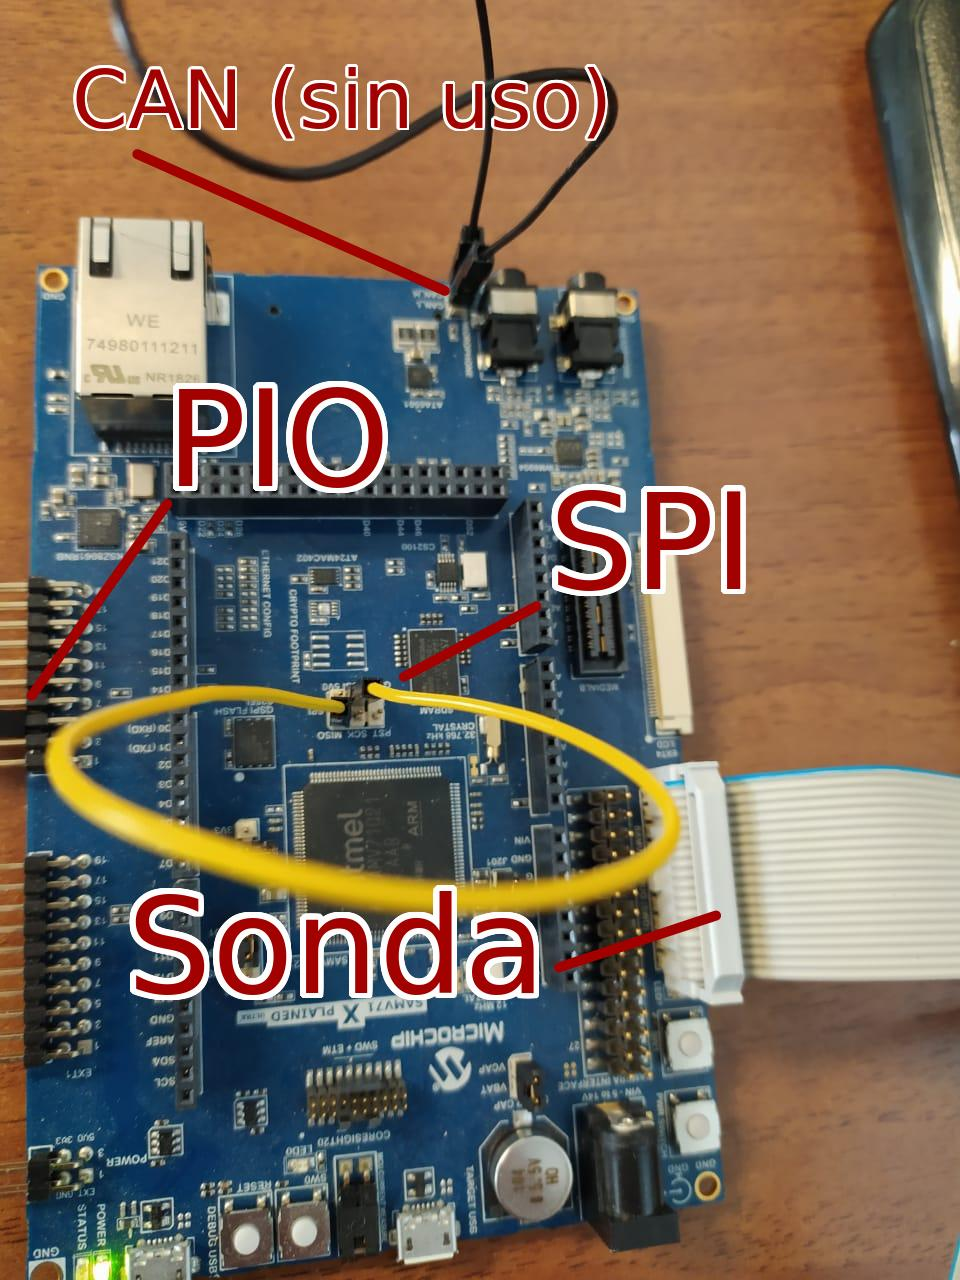
\includegraphics[width=\textwidth]{./Figures/labo.jpeg}
    \caption{Fotografía del dispositivo bajo prueba.}
	\label{fig:labo}
\end{figure}

Una vez configurados los componentes de \emph{hardware} del dispositivo bajo prueba; se procedió a diseñar el \emph{firmware}.
Se comenzó con la estructura que define los reportes de estado del dispositivo bajo prueba.
Los reportes están formados por 2 bytes, el primero es el carácter ``F'' y marca el inicio del reporte mientras que el segundo byte lleva la información del estado de los periféricos.
En el código \ref{cod:structs} se puede ver la implementación del segundo byte del reporte.

\begin{lstlisting}[language=C,label=cod:structs,caption=Definición de la estructura de reportes.]  % Start your code-block

#define BIT 1

struct status_bitfield_t
{
    uint8_t CAN:BIT;
    uint8_t SPI:BIT;
    uint8_t PIO:BIT;
    uint8_t WATCHDOG:BIT;
}__attribute__((packed));

typedef union
{
    struct status_bitfield_t status_of;
    uint8_t packed;
}report_t;

\end{lstlisting}

En el código \ref{cod:loop} se puede observar la implementación del lazo principal.
Es importante notar que en la línea 10 se utilizó la \emph{union} para transformar el reporte en caracteres legibles para una persona.
En la figura \ref{fig:firmwareflow} se puede observar el flujo completo del programa.

\begin{lstlisting}[language=C,label=cod:loop,caption=Lazo principal del \emph{firmware} de autoevaluación.]  % Start your code-block

while ( true )
{
    SYS_Tasks ( );
    report.status_of.CAN = validate_CAN();
    report.status_of.PIO = validate_PIO();
    report.status_of.SPI = validate_SPI();
    report.status_of.WATCHDOG = NORMAL;
    
    buffer[FRAME_START] = 'F';
    buffer[FLAGS_INDEX] = report.packed + 'A';
    USART1_Write(&buffer[0], FRAME_SIZE);
    
    WDT_Clear();
}

\end{lstlisting}

\begin{figure}[htbp]
	\centering
	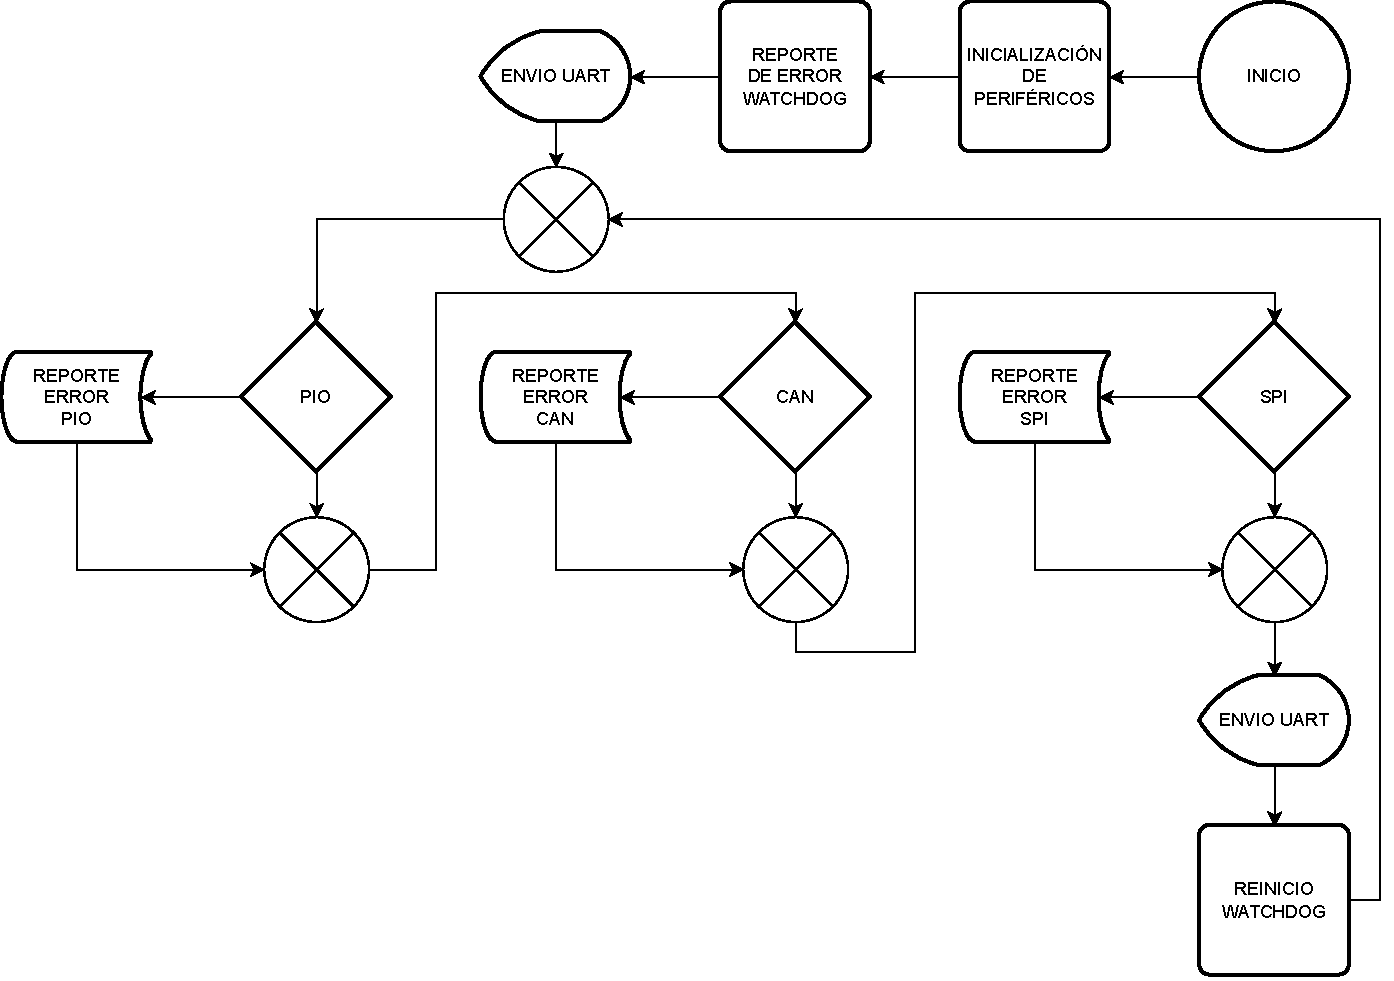
\includegraphics[width=\textwidth]{./Figures/firmwareflow.pdf}
    \caption{Flujo del \emph{firmware} de autoevaluación.}
	\label{fig:firmwareflow}
\end{figure}

\newpage

\section{Interfaz de programación de aplicaciones}
\label{sec:api}

% técnica RAII
% conexión como recurso
La interfaz de programación de aplicaciones tiene la función de abstraer al inyector de errores del servidor \emph{OCD}.
Esto se logró usando los siguientes patrones de diseño:

\begin{itemize}
    \item Programación orientada a objetos \emph{(OOP)}: este patrón de diseño se basa en agrupar en una unidad lógica las funcionalidades y estados que tengan un alto grado de acoplamiento.
        Esto significa que la funciones que tienen efectos colaterales junto a los datos mutados se encapsulan dentro de una construcción denominada objeto.
        El principal objetivo de un objeto es contener dentro suyo los efectos colaterales.
        Finalmente, el lenguaje de programación \emph{Python 3} permite, a través de una \emph{class}, modelar un tipo de dato que permite instanciar a un objeto.
    \item \emph{Resource Acquisition Is Initialization (RAII)}: este patrón de diseño consiste en modelar el ciclo de vida de un recurso al usar un objeto.
        Un recurso es todo aquello que requiera mantenimiento luego de su uso, como por ejemplo: liberar memoria, cerrar una conexión o unir dos hilos de programa.
        Esto se logra adquiriendo un recurso cuando se invoca el constructor de la \emph{class} por ejemplo, la conexión con la sonda de depuración se realiza durante la instanciación de un objeto llamado conexión.
        Luego, cuando se desea cerrar la conexión se invoca al destructor del objeto.
        Dentro de esta función se encuentra el código para cerrar de forma ordenada la conexión con la sonda y el dispositivo bajo prueba.
        Finalmente, este patrón de diseño hace que el programa maneje de forma robusta los recursos ya que está garantizada la ejecución de los destructores.
\end{itemize}

En el código \ref{cod:halted} se puede observar un ejemplo de \emph{RAII} donde se maneja como recurso la detención del núcleo del dispositivo bajo prueba.
Esto permite que frente una excepción del proceso que esté utilizando la interfaz de programación de aplicaciones, el núcleo pueda continuar operando.
Finalmente, se posibilita recuperar el proceso sin tener que reiniciar el dispositivo bajo prueba.

\begin{lstlisting}[language=Python,label=cod:halted,caption=Ejemplo de \emph{Resource Acquisition Is Initialization (RAII)}.]  % Start your code-block

class Halted():
    def __init__(self, target):
        self.target = target

    def __enter__(self):
        self.target.halt()

    def __exit__(self, exc_type, exc_val, traceback):
        self.target.resume()

\end{lstlisting}

Los patrones de diseño utilizados permiten escribir funciones expresivas y robustas.
Como se puede ver en el código \ref{cod:haltedexample}, es fácil comprender lo que sucede.
Se detiene el núcleo para leer una posición de memoria, luego de la lectura, el núcleo continua en funcionamiento.
Finalmente, se retorna el valor leído.

\newpage

\begin{lstlisting}[language=Python,label=cod:haltedexample,caption=Ejemplo de uso de \emph{RAII}.]  % Start your code-block

def readMemory(self, addr: int):
    with Halted(self.target):
        val = self.target.read_memory(addr)
    return val

\end{lstlisting}

En la tabla \ref{tab:funcionalidades} se puede observar un resumen de las funcionalidades y sus estrategias de abstracción.

\begin{table}[h]
	\centering
	\caption[Funcionalidades abstraidas]{Funcionalidades abstraídas}

	\begin{tabular}{l c c}    
		\toprule
        \textbf{Funcionalidad}     & \textbf{Patrón de diseño} & \textbf{Acceso}\\
		\midrule
		Conexión al integrado      & RAII                      & Público\\		
		Detener el núcleo          & RAII                      & Privado\\
		Registros CORE: read/write & OOP                       & Público\\
		Memoria SDRAM: read/write  & OOP                       & Público\\
		\bottomrule
		\hline
	\end{tabular}
	\label{tab:funcionalidades}
\end{table}

Finalmente, se logró abstraer el ciclo de vida de la sesión de depuración como se muestra en la figura \ref{fig:debugsession}.

\begin{figure}[htbp]
	\centering
	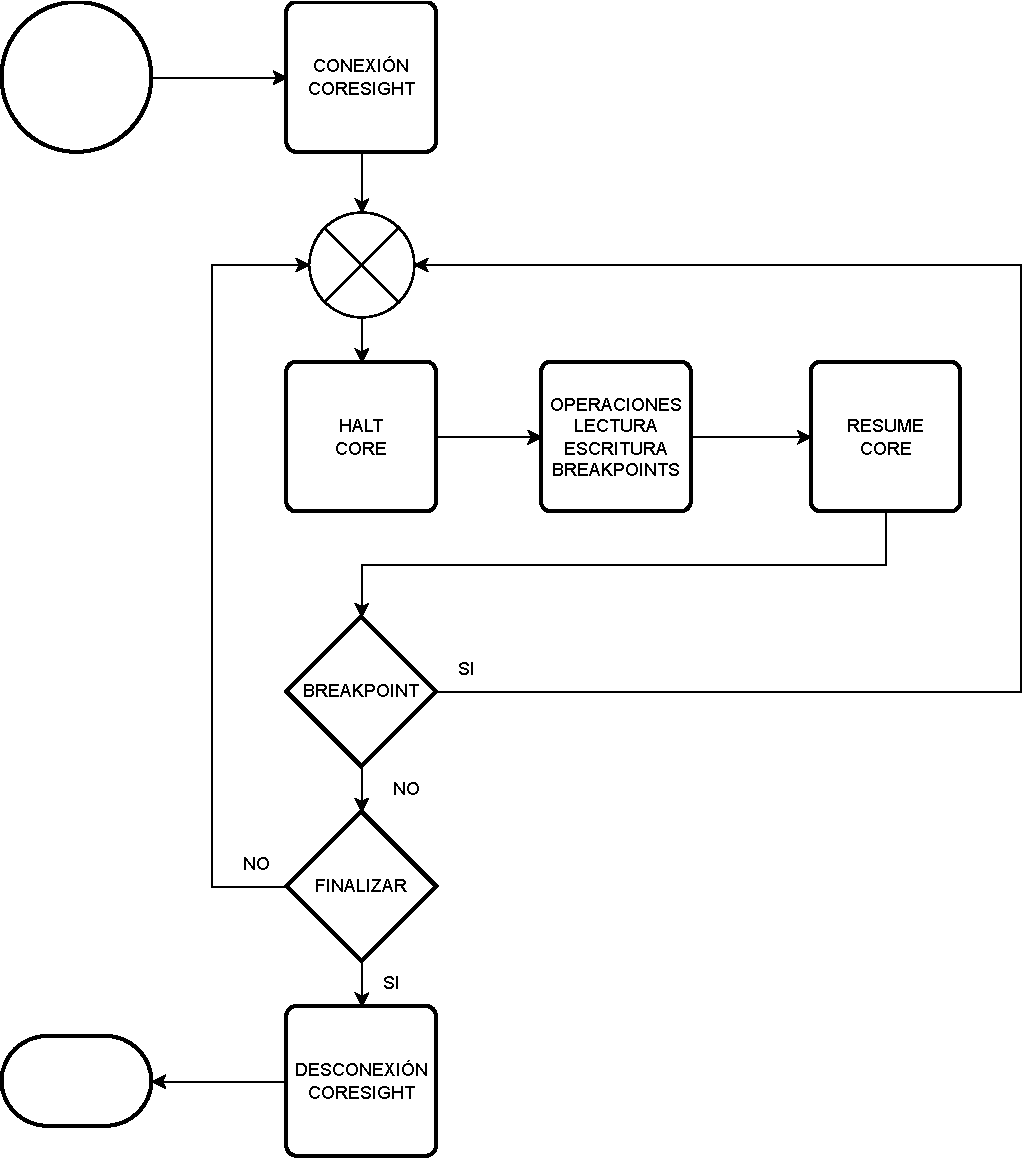
\includegraphics[width=0.9\textwidth]{./Figures/debugsession.pdf}
    \caption{Flujo de una sesión de depuración.}
	\label{fig:debugsession}
\end{figure}

\section{Sistema de inyección de emph{soft-errors}}
\label{sec:sise}

Una vez lograda la interfaz de programación de aplicaciones explicada en la sección \ref{sec:api}, se pudo construir el inyector por consola de comandos.

\begin{figure}[htbp]
	\centering
	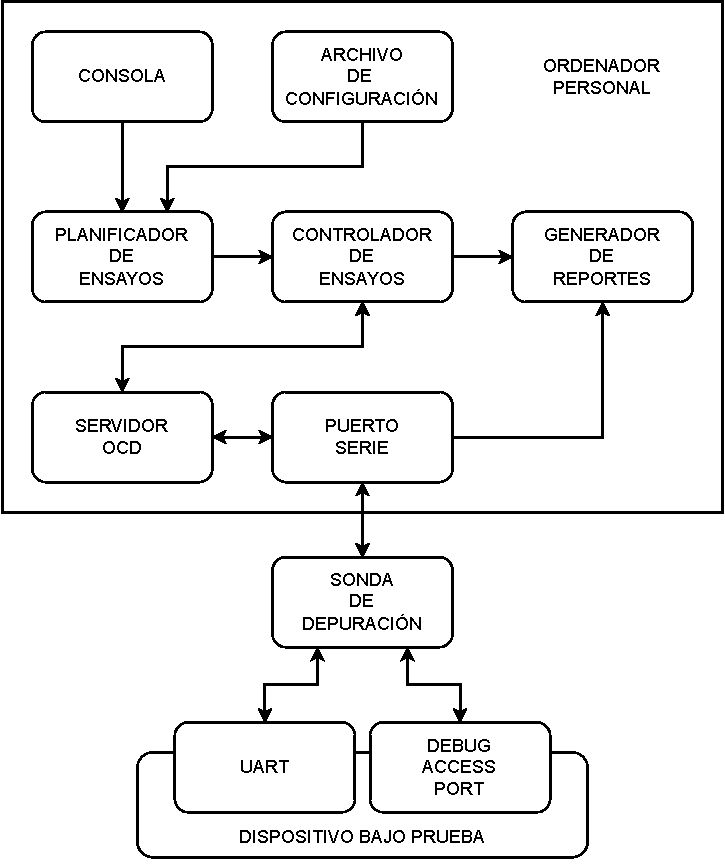
\includegraphics[width=\textwidth]{./Figures/siseblocks.pdf}
    \caption{Diagrama en bloques del sistema de inyección de soft-errors.}
	\label{fig:siseblocks}
\end{figure}

\begin{figure}[htbp]
	\centering
	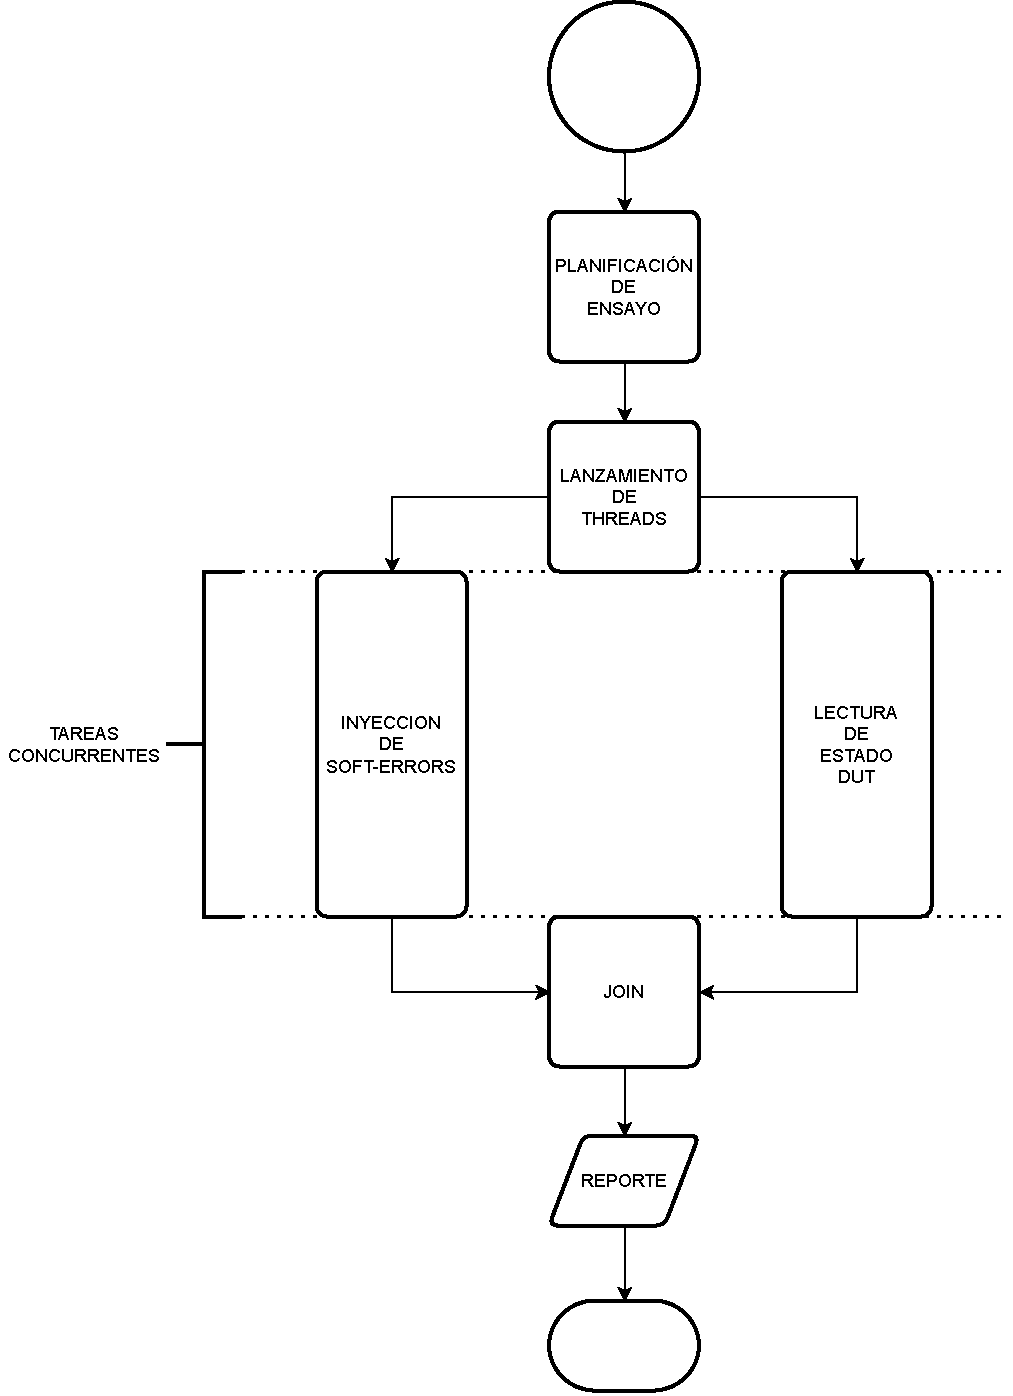
\includegraphics[width=\textwidth]{./Figures/concurrencia.pdf}
    \caption{Flujo de tareas concurrentes.}
	\label{fig:concurrencia}
\end{figure}

\begin{figure}[htbp]
	\centering
	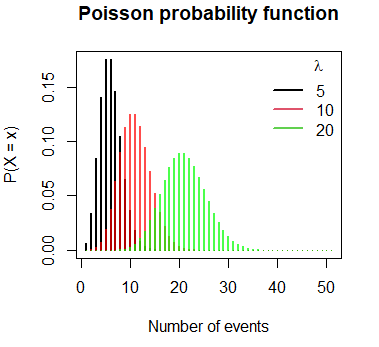
\includegraphics[width=0.7\textwidth]{./Figures/poisson.png}
    \caption{Gráfico de distribución Poisson\citep{WEBSITE:poisson}.}
	\label{fig:poisson}
\end{figure}

\section{Biblioteca para el desarrollo de ensayos}
\label{fig:biblioteca}

\begin{lstlisting}[language=Python,label=cod:vControl,caption=Ejemplo de aplicación de la biblioteca.]  % Start your code-block

import sise.library as sise

dut = sise.Connection()

# Bit-flip en SDRAM
addr = 0x20400000
bit = 0
res = dut.bitFlipMemory(addr, bit)
print("res:", res)

del(dut)

\end{lstlisting}
